\section{What this means}
\label{sec:discussion}

\paragraph{In our runs, programming compiled rather than learned.} We began by asking whether weight-space programming can only redirect what a model knows. It can do more: it can add knowledge. But it adds knowledge in a particular way. In every case where programming beat fine-tuning, the programmer turned the training labels into an explicit object and wrote that object into the weights:
\begin{itemize}
  \item a swapped pair of words (SST-5 inverted);
  \item a table of facts (fictional facts);
  \item a table of answer rates (Twin-2K).
\end{itemize}
Nothing was learned in the sense that fine-tuning learns, by gradually shaping features until they generalise. A compiler can only compile what can be written down. That explains both the strengths and the ceiling. Programming did best where the target is a short rule or a finite table, and worst on SST-5, where it is neither: three independent programmers found three mechanisms and hit the same ceiling.

\paragraph{The knowledge map, and what the probe misses.} Figure~\ref{fig:map} places every method on one chart. For edits that work through the model, the gain roughly tracks the probe's headroom: large where the model holds an unused answer, small where it does not. The probe predicted the redirect regime on both models. It does not predict compiling. Bypass circuits and the Opus memory gain 56--79 points on facts, where the probe finds nothing, and LoRA gains twelve points on Twin-2K, where the probe again finds nothing. A linear probe at one position estimates what a \emph{readout} edit can use. It does not estimate what a programmer who builds new machinery, or a gradient that trains it, can reach. Deciding which regime a task is in therefore still needs judgement. One test is whether the target can be written down from the labels.

\begin{figure}[t]
\centering
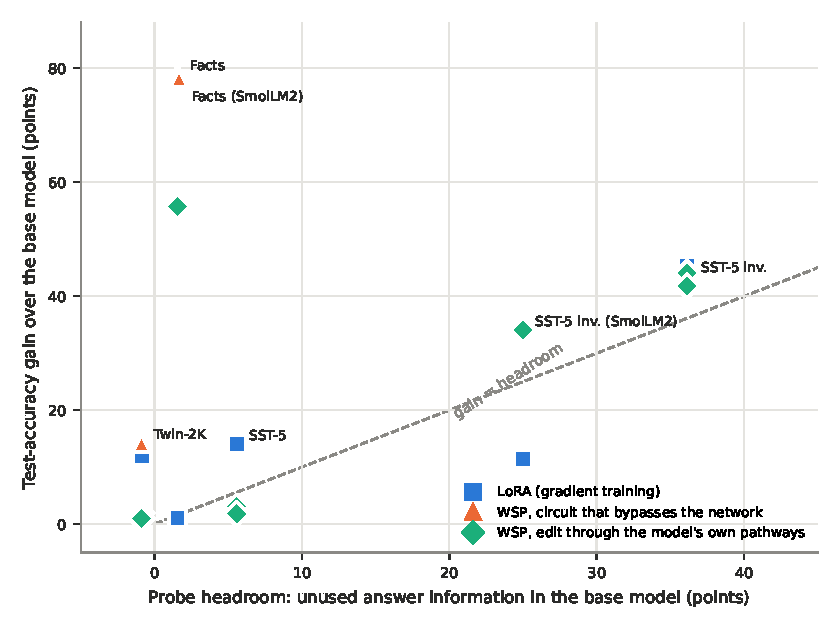
\includegraphics[width=0.75\linewidth]{figures/knowledge_map.pdf}
\caption{The knowledge map: gain over the base model against probe headroom, for every method on both models (test points; preserve runs omitted). Edits through the model's pathways (green) roughly follow the diagonal, recovering about as much as the probe says is unused. Compiled edits (orange, and the Opus facts memory at upper left) sit far above it: they add knowledge the probe says is absent. LoRA (blue) gains on most tasks regardless of headroom, but fails on SST-5 inverted for SmolLM2 and on facts at the default budget.}
\label{fig:map}
\end{figure}

\paragraph{Around or through decides the cost, and the brief decides which.} The finding with the most practical weight concerns side effects. The same information can be written into a model in a way that leaves it intact or one that wrecks it, depending on whether the edit goes around the network or through it.
\begin{itemize}
  \item \textbf{Bypass circuits} are easier to make exact, because the programmer controls every step, so they score highest. But they claim components every input depends on, and their output overwhelms the rest of the computation. On both model families, they left the model at chance on general knowledge.
  \item \textbf{Through edits} have to cooperate with what the network already does, so they are less exact and far less destructive. Fine-tuning is a through edit by construction.
\end{itemize}
The preserve experiment shows the choice belongs mainly to the instruction, not the method. The same programmer that built three destructive facts circuits under the standard brief built a gated, intact edit for Twin-2K when told to preserve the model. It did not manage one for facts, so preservation sometimes costs everything that was gained. This qualifies the conclusion of \citet{yang2026writing} that written edits disturb less: their one published patch was gentler than LoRA, but here the most accurate written edits were far more destructive than LoRA. How gentle an edit is depends on how it is built, not on whether it is written or trained.

\paragraph{How to evaluate an edit.} Two traps appeared, pointing in opposite directions.
\begin{itemize}
  \item \textbf{Target-task accuracy rewards the most damaging edits.}
  \item \textbf{Raw perplexity punishes harmless ones,} because a temperature change multiplies it a hundredfold without changing a single prediction.
\end{itemize}
A minimal protocol that avoided both in our study has four checks:
\begin{itemize}
  \item next-token top-1 accuracy on ordinary text;
  \item a general-knowledge benchmark;
  \item a task unrelated to the edit;
  \item consistency under option reordering.
\end{itemize}
The first three separated bypass from through edits without exception. The last shows whether an edit changed what the model reads or how it reads.

\paragraph{Program first, then fine-tune.} The most useful practical result is that the two methods combine. Fine-tuning failed in two ways that a programmed edit fixed:
\begin{itemize}
  \item \textbf{Slow storage of new facts.} The edit cut the training needed by up to tenfold.
  \item \textbf{A stall on a confidently wrong start.} The edit removed the plateau that stopped two of three seeds on Qwen and all three on SmolLM2. On Qwen, LoRA alone needed three times the data to get past it; we did not try more data on SmolLM2.
\end{itemize}
In return, fine-tuning took each edit far past its own ceiling, and the combined models kept general ability. On SST-5 inverted, the part of the edit that mattered is a two-row swap anyone could write once they know the readout is mirrored; the programmer's contribution was finding it without being told. This suggests a workflow. A programmer inspects the model and writes a small, readable edit for whatever can be redirected or compiled, which takes minutes of GPU time (though \$16--\$86 of programmer API time for a typical run, at list prices), and gradient training does the rest. The edit also documents what the model was missing.

\paragraph{A rule of thumb.} Table~\ref{tab:guide} condenses the results into a choice of tool.

\begin{table}[h]
\centering\small
\begin{tabular}{p{4.4cm}p{3.6cm}p{5.8cm}}
\toprule
If the problem is\ldots & Reach for\ldots & Because\ldots \\
\midrule
The model knows the answer but reads it out wrongly (a flipped label, a misrouted feature) & Weight-space programming, then fine-tuning & Tiny, readable, reproducible edits match fine-tuning, are more reliable, and need fewer labels. Fine-tuning on top adds about ten points (SST-5 inverted). \\
\addlinespace
The model must recall a table and does nothing else & Either; programming is faster on GPU & A compiled lookup matched or beat fine-tuning (facts, Twin-2K). \\
\addlinespace
The model must recall a table \emph{and} keep its other abilities & A programmer told to work through the model's pathways, then fine-tuning & Bypass circuits destroyed general ability; through edits and LoRA did not. An edit plus LoRA reached 99\% with a tenth of LoRA's data and kept general ability. \\
\addlinespace
The model must get better at a mapping it already partly does & Fine-tuning & Programming gained about three points where LoRA gained fourteen, and LoRA still gained nine with only 256 examples (SST-5). \\
\bottomrule
\end{tabular}
\caption{When to program and when to fine-tune, based on our results with 1.5--1.7B models.}
\label{tab:guide}
\end{table}

\paragraph{The programmer matters most when there is something to build.} Two programmer models were equally good at redirection, but the stronger one was much better whenever an edit had to be constructed, and it was also the one that took the destructive route. If programming is compiling, this is what one would expect: the output depends on the engineer, and on the specification the engineer is given. It also means results will change as programmer models improve. Our findings describe what current models do with this budget, not a limit of the method.

\paragraph{A note on simulating people.} Twin-2K adds a finding that matters outside this comparison. Neither fine-tuning nor programming beat the plain per-question answer prior, which ignores the person entirely. The best programmed edit was that prior in circuit form. For a 1.5B model, a person's profile added nothing measurable over knowing what people in general answer. Work that claims to simulate individuals with language models should report this prior as its baseline. A model that beats chance but not the prior is simulating a population.
